%%%%%%%%%%%%%%%%%%%%%%%%%%%%%%%%%%%%%%%%%%
% CHAPTER 1 SIMPLE HARMONIC MOTION
%%%%%%%%%%%%%%%%%%%%%%%%%%%%%%%%%%%%%%%%%%

\chapter{Simple Harmonic Motion}
\marginnote{\emph{Lecture 1}\\
\noindent \S Suggested Reading:
\begin{itemize}
\item \emph{Pain}, Chapter 1, Simple Harmonic Oscillators
\item \emph{Tipler}, Chapter 14, Oscillations
\end{itemize}
}
\section*{Introduction}
\emph{Periodic motion} is motion of an object that regularly repeats, i.e. the object returns to a given position after a fixed time interval.
\begin{examplebox}{Examples of Periodic Motion}
\begin{itemize}[noitemsep]
\item{\p{Orbital motion of the Earth;}}
\item{\p{Orbital motion of the moon;}}
\item{\p{Vibrations of Molecules in a solid;}}
\item{\p{Electromagnetic Waves (light);}}
\item{\p{Loudspeakers;}}
\item{\p{Oscillations of Bridges;}}
\item{\p{Swaying of Tall Buildings.}}
\end{itemize}
\end{examplebox}
A very important kind of periodic motion is \emph{Simple Harmonic Motion (SHM)}. In a certain sense, SHM describes the simplest possible periodic motion. Understanding SHM well can lead to a physical understanding of all kinds of dynamical systems, such as those in the examples above. 

\section{Mechanics of Simple Harmonic Motion}
In oscillating mechanical systems there is always a force that acts to reduce displacement of an object and return the system to equilibrium. This force is called the \emph{restoring force}, $F_r$.
 
\begin{mybox}{Simple Harmonic Motion}
\emph{SHM} occurs whenever the restoring force is linearly proportional to the displacement from equilibrium and opposite to the direction of the displacement, i.e. 
\begin{align}
\vec{F}_r \propto - \vec{x}. 
\end{align}
\end{mybox}
Any (stable) system that oscillates, \emph{if the oscillation is small enough}, will appear to be undergoing simple harmonic motion. 

%\marginnote[0.5cm]{
%Model
%\begin{enumerate}
%	\item{no friction;}
%	\item{mass of spring is negligibly small in comparison with the mass of the block;}
%	\item{spring only responds linearly;}
%\end{enumerate}
%}
\pagebreak
\begin{figure}[h!]
\pincludegraphics{L1/Fig1_1_blank.pdf}{L1/Fig1_1.pdf}
\caption{In this model our assumptions are: \emph{(1)} There is no friction; \emph{(2)} The mass of spring is negligibly small in comparison with the mass of the block; \emph{(3)} The spring only responds linearly.}
\label{Fig1_1}
\end{figure}

Consider the mass $m$ attached to a spring, shown in Figure \ref{Fig1_1}. When the mass is \emph{in equilibrium} there is no (net) force on it. When the mass is displaced, the spring exerts a \emph{restoring force} $-kx$, as given by \emph{Hooke's Law} \marginnote{Hooke's Law}
\begin{align}
\p{F_r = -kx}
\end{align} 
where $k$ is the constant of proportionality between the displacement and the restoring force, called the \emph{spring constant} (or \emph{force constant}).

The minus sign in Hooke's law arises because the force is in the opposite direction of the displacement. 

Using Newton's Second Law of Motion we get
\begin{align}
\vec{F}(x) = m \vec{a}(x) \qquad \textrm{or}\qquad -k\vec{x} = m \vec{a} \label{eq:SpringEoM}
\end{align} 

This can be written as
\begin{align}
\p{\frac{d^2 \vec{x}}{dt^2}} &\p{= - \frac{k}{m} \vec{x}}
\end{align}
If we calculate the dimensions of $k/m$\marginnote[-0.5cm]{\p{The spring constant has units of [Mass][Time]$^{-2}$, therefore $ \omega^2 \equiv k/m$ has units of $1/$[Time]$^2$}} then we find it has the dimensions of $[\textrm{Time}]^{-2}$ so we can write,\marginnote[1cm]{The differential equation for SHM}
\begin{align}
\p{\frac{d^2 x}{dt^2} + \omega^2 x} &\p{= 0} \label{SHM_DE} \\
\p{\ddot{x} + \omega^2 x} &\p{= 0}  \nonumber
\end{align}
where $\omega = \sqrt{k/m}$ is an \emph{angular frequency}.

Equation \eqref{SHM_DE} is a second order differential equation. It is often referred to as the \emph{differential equation of Simple Harmonic Motion}. 

Its solution can always be written in the form, \marginnote[1cm]{\p{Note that if $\delta$ gives the initial phase for some SHM, so can $\delta + 2\pi N$ where $N$ is some integer. $\delta$ is not unique because the solution is periodic!}}

\begin{align}
\p{x = \underbrace{A}_{\textrm{Amplitude}} \cos(\overbrace{\omega t + \underbrace{\delta}_{\textrm{Initial Phase}}}^{\textrm{Phase}})} \label{SHM_sol}
\end{align}
where $A$ and $\delta$ are determined by the initial conditions (i.e. the displacement and velocity at $t = 0$). 
According to Eq. \eqref{SHM_sol}, the function $x(t)$ has the form:
\begin{figure}
\pincludegraphics{L1/Fig1_2_blank.pdf}{L1/Fig1_2.pdf}
\caption{\emph{Units:} Period $T$ is in 'seconds'; Frequency $f = 1/T$ is in 'Hertz'; Angular frequency $\omega = 2\pi f$ is in 'radians per second'; and initial phase $\delta$ is in 'radians'.}
\end{figure}

The period of the oscillation $T$ is given by \marginnote[1cm]{Period in terms of angular frequency}
\begin{align}
T = \frac{2\pi}{\omega}.
\end{align}

\section{Displacement, Velocity, and Acceleration}
If we have the solution $x = A \cos(\omega t + \delta)$, then the velocity is 
\marginnote[0.5cm]{%
SHM solutions for $x$, $v$, and $a$.\\ 
\p{Remember the chain rule: 
\begin{align}
\frac{df(g(t))}{dt} &= \frac{df}{dg} \cdot \frac{dg}{dt} \nonumber\\
\frac{dx}{dt} &= A\underbrace{\frac{d [\cos(\omega t + \delta)]}{d(\omega t + \delta)}}_{-\sin(\omega t + \delta)} \underbrace{\frac{d(\omega t + \delta)}{dt}}_{\omega}\nonumber
\end{align}}
}
\begin{align}
\p{v = \frac{dx}{dt} = - A \omega \sin(\omega t + \delta)}
\end{align}
and the acceleration is  \marginnote[0.5cm]{\p{We can check to see that the solution's acceleration and displacement indeed satisfy the original SHM differential equation}
\begin{align}
\p{\ddot{x} + \omega^2 x} &\p{= 0} \nonumber \\
\p{-A \omega^2 \cos(\omega t + \delta) + \omega^2 A \cos(\omega t + \delta)} &\p{= 0} \nonumber
\end{align}
}
\begin{align}
\p{a = -A\omega^2 \cos(\omega t + \delta) = -\omega^2 x}
\end{align}

For initial phase $\delta = 0$, the equations simplify to:\begin{subequations}
\begin{align}
x &= A \cos \omega t\\
v &= -\omega A \sin \omega t\\
a &= -\omega^2 A \cos \omega t = -\omega^2 x. \label{a_delta0}
\end{align}
\end{subequations}

\pagebreak
Let's plot out the above solutions for $x(t)$ assuming $\delta = 0$:

\begin{figure*}[h!]
%\ifthenelse{\boolean{skeletal}}{
%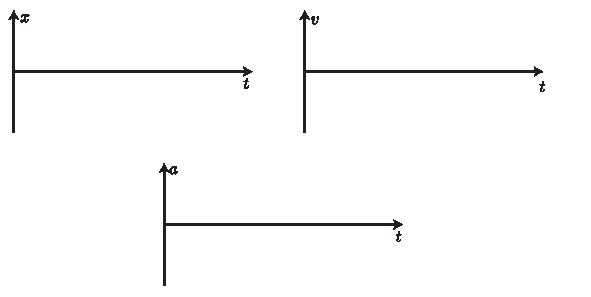
\includegraphics{./L1/Fig1_3_blank.pdf}
%}{
%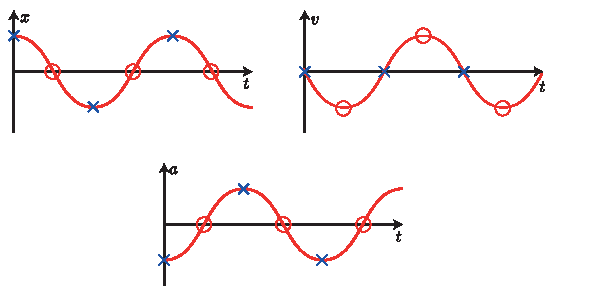
\includegraphics{./L1/Fig1_3.pdf}
%}
\pincludegraphics{./L1/Fig1_3_blank.pdf}{./L1/Fig1_3.pdf}
\caption{Position, Velocity and Acceleration for SHM with $\delta = 0$.}
\end{figure*} 
\begin{itemize}
\item Velocity is $\pi/2$ out of phase with displacement. 
\item \textcolor{red}{o} - velocity is maximum/minimum when displacement is zero. 
\item \textcolor{blue}{x} - Velocity is zero when displacement is maximum/minimum. 
\item Acceleration is proportional to displacement and acts in the opposite direction to the displacement.
\end{itemize}

Note that the \emph{minimum} isn't the zero point. The displacement, velocity, and acceleration oscillate about zero, \emph{the equilibrium point}. 

The \emph{frequency} and \emph{period} are related to the \emph{stiffness} $k$ of the spring and the \emph{mass} of the particle\marginnote[1cm]{$f$ and $T$ in terms of $k$ and $m$ for a SHM}
\begin{align}
f = \p{\frac{1}{2\pi} \sqrt{\frac{k}{m}}} \qquad \textrm{and} \qquad T = \p{2\pi \sqrt{\frac{m}{k}}}
\end{align}
Note that the \emph{spring consant} $k$ is only a constant for small displacements. 

Large displacements could cause (for example) permanent deformation of the spring and the system would not oscillate with SHM. This reminds us that the SHM is only found for small displacements. 

\pagebreak
\begin{examplebox}[width = \pagewidth]{An air-track glider}
An air-track glider attached to a spring oscillates with a period of 1.5s. At $t = 0$ the glider is 5cm left of the equilibrium position and moving to the right at 36.3 cm/s.
\begin{enumerate}[label=(\alph*)]
\item What are the amplitude and initial phase of the oscillations?
\item Write down an expression that describes the position of the glider as a function of time
\item What is the glider's position at $t = 0.5$s?
\end{enumerate}
\p{We know that the glider undergoes SHM, with solution}
\p{\begin{align}
x = A \cos(\omega t + \delta) \nonumber
\end{align}}
\p{We need to know $\omega$, $A$, and $\delta$ in order to completely describe the motion. For $\omega$ we have, 
\begin{align}
\omega = \frac{2\pi}{T} = \frac{2\pi}{1.5 \textrm{s}} = \frac{4\pi}{3} \textrm{rad/s} = 4.2 \textrm{rad/s} \nonumber
\end{align}}

\p{\begin{enumerate}[label=(\alph*)]
\item{At $t = 0$ we have 
\begin{align}
x(0) &= A \cos( 0 + \delta) = A \cos \delta = -5 \textrm{cm}\nonumber\\
v(0) &= -A \omega \sin (0 + \delta) = - A \omega \sin \delta = 36.5 \textrm{cm/s}\nonumber
\end{align}
Dividing $v(0)$ by$x(0)$, we can find $\delta$,
\begin{align}
\frac{v(0)}{x(0)} &= - \frac{A \omega \sin \delta}{A \cos \delta} = -\omega \tan \delta = \frac{36.5\textrm{cm/s}}{-5 \textrm{cm}}\nonumber\\
\tan \delta &= 1.734\nonumber\\
\Rightarrow \delta &= \pi/3 \textrm{ rad} = 60^\circ\nonumber
\end{align}
Finally, from the expression for $x(0)$ above, we can find $A$
\begin{align}
A &= \frac{x(0)}{\cos \delta} = \frac{-5 cm}{0.5} \nonumber\\
\Rightarrow A &= -10 \textrm{cm} \nonumber
\end{align}
}
\item{%
\begin{align}
x(t) &= A \cos (\omega t + \delta)\nonumber\\
\Rightarrow x(t) &= -10 \cos \left(\frac{4\pi}{3}t + \frac{\pi}{3}\right) \nonumber
\end{align}
}
\item{%
\begin{align}
x(0.5 \textrm{s}) &= -10 \cos( \underbrace{(4 \pi/3)\cdot 0.5}_{2\pi/3 \textrm{ rad} = 120^\circ} + \pi/3) = - 10 \underbrace{\cos \pi}_{-1} \nonumber \\
\Rightarrow x(0.5 \textrm{s}) &= 10 \textrm{cm} \nonumber
\end{align}
}
\end{enumerate}}
\end{examplebox}
\marginnote[1cm]{\emph{End of Lecture 1}}

